\section{Conclusions}\label{sec:Conclusion}

The calibration of LArIAT's data and Monte Carlo samples over the Run-I and Run-II periods using the Bethe-Block description of the mean rate of energy loss for various particle species allows us to calibrate the dE/dX response for various samples.

In this note, we showed the calibration using negative and positive polarity data for samples of $\pi, \mu, e$ and protons and cosmic rays as well using pion and proton Monte Carlo.

The calibration constants derived for the various run periods and Monte Carlo are summarized as:

\begin{itemize}
\item \textbf{Run-I}: \verb!physics.producers.calo.CaloAlg.CalAreaConstants: [0.032,0.058]!

\item \textbf{Run-II}: \verb!physics.producers.calo.CaloAlg.CalAreaConstants: [0.021,0.0490]!

\item \textbf{Monte Carlo}: \verb!physics.producers.calo.CaloAlg.CalAreaConstants: [0.094, 0.101]!
\end{itemize}


Figure \ref{fig:PionCompareDataAndMC} shows the direct comparison of the dE/dX distribution for Run-I DDMC and Run-I $\pi, \mu, e$ data. With the tuning of the calibration constants, they agree in both MPV and shape. 

\begin{figure}[htb]
\centering
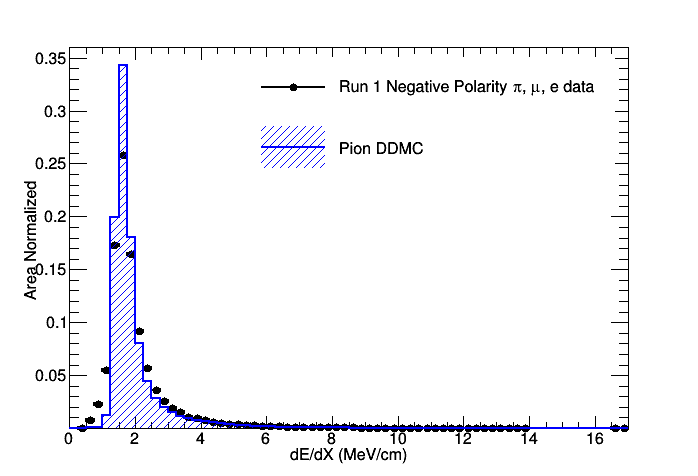
\includegraphics[width=0.48\textwidth]{images/dEdXPionDataMCcompare.png}
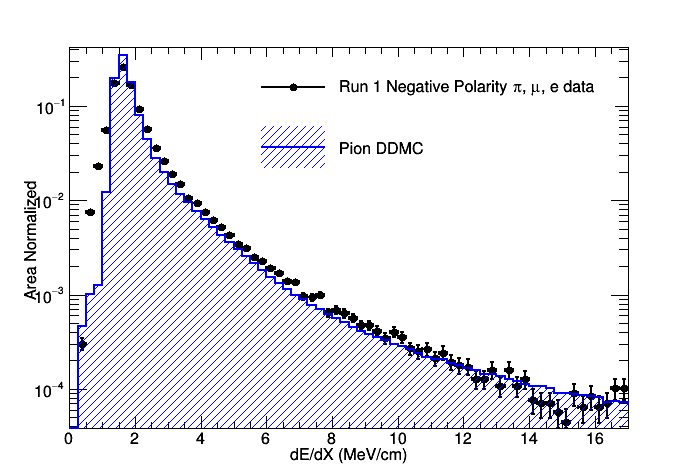
\includegraphics[width=0.48\textwidth]{images/dEdXPionDataMCcompareLog.png}
\caption{Comparison of the dE/dX distributions for Pion DDMC and Run-I Negative Polarity $\pi, \mu, e$ data. The distributions have been area normalized, the left hand side is the linear y-axis scale while the right hand side is the log scale for the y-axis.}
\label{fig:PionCompareDataAndMC}
\end{figure}

